\documentclass[12pt]{article}
\usepackage{fullpage,amsmath,amssymb,graphicx}

\usepackage{setspace}
\spacing{1}

\usepackage{textpos}
\usepackage{tikz}
\usepackage{pgf}
\usepackage{amssymb}
\usepackage{enumerate}
\usepackage{xcolor}
\usepackage{graphicx}
\usepackage{subcaption}
\usepackage{tabularx}
\usepackage{colortbl}
\usepackage{multicol}
\usepackage{longtable}
\usepackage{hyperref}


\definecolor{encabezado}{rgb}{0.74, 0.83, 0.9}

\begin{document}

\hfill\\
\rule{\textwidth}{1.5pt}

\begin{minipage}[t]{85mm}
  \begin{tabular}{l}
    \textbf{\large Instituto Tecnológico de Costa Rica} \\  
    \textbf{Escuela de Ingeniería Electrónica} \\
    \textbf{Trabajo Final de Graduación} \\
    \textbf{Proyecto:} Método basado en aprendizaje reforzado \\para el control automático de una planta no lineal. \\
    \textbf{Estudiante:} Oscar Andrés Rojas Fonseca \hspace{3cm}\rule{4.5cm}{1.5pt}\\
    I Semestre 2024 \hspace{8.5cm}\textbf{Firma del asesor}
  \end{tabular}
\end{minipage}
\hfill\\
\rule{\textwidth}{1.5pt}


\section*{Bitácora de trabajo}

%\begin{table}[h]
\begin{minipage}[h]{\textwidth}
	\centering
	\begin{tabularx}{\textwidth}{|p{2cm}|X|X|p{2cm}|} 
		\hline
		\rowcolor{encabezado}
		\textbf{Fecha} & 
		\textbf{Actividad} & 
		\textbf{Anotaciones} & 
		\textbf{Horas dedicadas} \\ \hline
		% ***************************************************************
		12/02/2024 & 
		$\mathbf{1}.$ Búsqueda de repositorios en línea sobre RL. & 
		$a)$ Se encontró la librería \textit{RLtools} en C++. . \newline $b)$ Creación del env para trabajar con C++. \newline $c)$ Ejemplo de implementación de \textit{RLtools}. \newline  & 
		4 horas \\
	 	% ***************************************************************
	 	13/02/2024 & 
	 	$\mathbf{2}.$ Búsqueda de ejemplos de uso del modelo \textit{Mamba}. &
	 	$a)$ Se encontraron ejemplos de funcionamiento con \textit{simple parallel scan implementation}. \newline $b)$ Estudio de la comparación entre el entrenamiento Mamba con \textit{CUDA}, \textit{mamba.py} y \textit{RNN}. \newline $c)$ El repositorio $mamba.py$ encontrado ejempifica un uso simple de MAMBA. \newline & 
	 	5 horas \\
	 	% ***************************************************************
	 	13/02/2024 & 
	 	$\mathbf{3}.$ Trabajo en la tesis del proyecto. & 
	 	$a)$ Se adaptó la plantilla para el proyecto. \newline $b)$ Introducción de línea guía de ideas (anteproyecto). \newline $c)$ Introducción de resumen de la bitácora semana 1. \newline & 
	 	3 horas \\
	 	
	 	\hline
	\end{tabularx}
\end{minipage}	 	
	 	
	 	% ***************************************************************
\hfill\\
\begin{minipage}[h]{\textwidth}
	\centering
	\begin{tabularx}{\textwidth}{|p{2cm}|X|X|p{2cm}|} 
		\hline		
		
	 	15/02/2024 & 
	 	$\mathbf{4}.$ Revisión del funcionamiento del código $RNAM\_ Synthetic.py$. & 
	 	$a)$ Primer proceso de entrenamiento de la versión base. \newline 
	 	$b)$ Se verificó el registro con lo expuesto en la tesis de Jorge Brenes. \newline 
	 	$c)$ Se probó el código de $RNAM\_ Real.py$ sin exito por la falta del directorio $../Datos\_ Recolectados/..$. \newline & 
	 	6 horas \\
	 	% ***************************************************************
	 	16/02/2024 & 
	 	$\mathbf{5}.$ Pruebas de variación de hiperparámetros al entrenamiento. & 
	 	$a)$ Cambios en el valor del $learning\_ rate$.\newline & 
	 	3 horas \\
	 	% ***************************************************************
	 	\hline
		\multicolumn{3}{|r|}{Total de horas de trabajo:} & 21 horas \\ 
	 	\hline                 
	\end{tabularx}
\end{minipage}
%\end{table}

% *****************************************************************************
% *****************************************************************************
% *****************************************************************************
\newpage

\section*{Contenidos de actividades}

\subsection*{Resumen de repositorios encontrados}

El ejemplo más completo corresponde a la librería encontrada \textit{RLtools} \cite{rltools}, la cual cuenta con una descripción muy completa de lo que puede ofrecer al tabular y compartir capturas del entrenamiento de modelos de RL mediante algoritmos como \textit{Twin Delayed DDPG} ($TD3$), \textit{Proximal Policy Optimization} (PPO) y \textit{Soft Actor-Critic} (SAC).

Se muestran ejemplos de implementación con casos como \textit{Pendulum}, \textit{Racing car}, \textit{MujoCo Ant-man} and \textit{Acrobot} \cite{rltools}, similares a las capturas de la Figura \ref{fig:rltools}.

\begin{figure}[h]
	\centering
	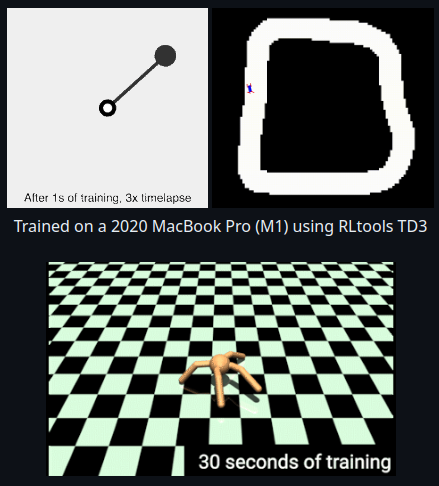
\includegraphics[scale=0.5]{Fig/RLtools.png}
	\caption{Capturas de implementación con RLtools \cite{rltools}.}
	\label{fig:rltools}
\end{figure}

De igual forma se encontró el repositorio de la librería \textit{mpcrl} en python \ref{fig:rlfigs}, para el entrenamiento de RL basado en modelos. La descripción del \textit{README.md} es completa y se acompaña con ejemplos de funcionamiento y la captura facilitada mostrada en la Figura \ref{fig:rlfigs}.

\begin{figure}[h]
	\centering
	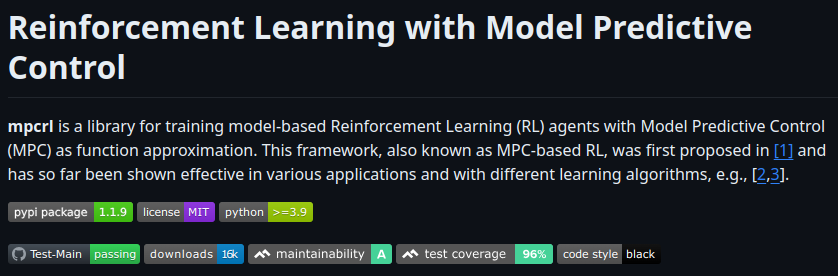
\includegraphics[scale=0.35]{Fig/Jucs.png}
	\caption{Capturas de descripción del modelo \cite{}.}
	\label{fig:rlfigs}
\end{figure}

Para la búsqueda realizada para los repositorios de Mamba, se encontró el caso de \cite{mamban}, donde si se cuenta con implementación de Mamba, pero se trata de una ejemplificación de cálculos sencillos mediante PyTorch y en diferentes métodos para implementación.


\begin{figure}[h]
	\centering
	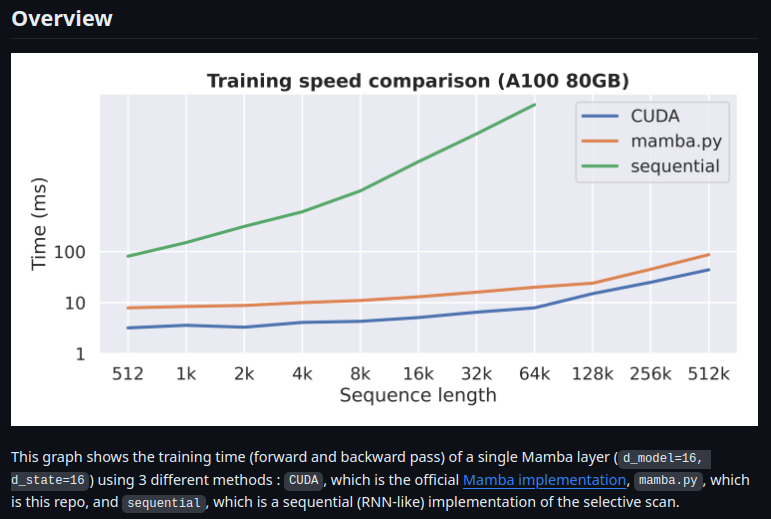
\includegraphics[scale=0.35]{Fig/mamban.png}
	\caption{Capturas de la descripción del modelo Mamba \cite{mamban}.}
	\label{fig:mamban}
\end{figure}




\newpage

\section*{Referencias}
\renewcommand\refname{}
\bibliographystyle{IEEEtran}
\bibliography{references}





\end{document}